
\subsection{Data}
This measurement uses the full dataset of 2016 collected with the CMS detector in pp collisions
at 13 TeV center-of-mass energy with the corresponding integrated luminocity of 35.9 ~\fbinv. 

As the measurement is based on dilepton signatures, the DoubleMuon and DoubleElectron primary
datasets are analyzed and only on-shell \Zll~decays are considered, where $\ell=\Pe, \Pgm$.
 
The run periods and the corresponding integrated luminosities are listed in Table ~\ref{tab:datasets} for DoubleMuon channel, DoubleElectron channel numbers are similar.
\begin{table}[htbp]
\caption{List of used 2016 DoubleMuon data sets.
%\lumi16  across all modes.  
An uncertainty of $2.5\%$ is  assigned for the 2016 data set luminosity~\cite{lumiUnc}}

\label{tab:datasets}
\begin{center}
\scalebox{0.9}{
\begin{tabular}{|c|c|} \hline%\hline
Dataset       & $\int\cal L$ (\fbinv) \\
\hline
%{\tt DoubleMuon\_Run2016B-03Feb2017-v1}       & \multirow{2}{*}{$\sim$5.9}  \\
{\tt DoubleMuon\_Run2016B-03Feb2017-v2}       & {$\sim$5.9}  \\
%{\tt DoubleMuon\_Run2016B-03Feb2017-v2}       &   \\
{\tt DoubleMuon\_Run2016C-03Feb2017-v1}       & $\sim$2.7 \\
{\tt DoubleMuon\_Run2016D-03Feb2017-v1}       & $\sim$4.3 \\
{\tt DoubleMuon\_Run2016E-03Feb2017-v1}       & $\sim$4.1 \\
{\tt DoubleMuon\_Run2016F-03Feb2017-v1}       & $\sim$3.2 \\
{\tt DoubleMuon\_Run2016G-03Feb2017-v1}       & $\sim$3.8 \\
{\tt DoubleMuon\_Run2016H-03Feb2017-v1}       & $\sim$11.8 \\
\hline
Total Lumi                        & 35.9 \\
\hline%\hline
\end{tabular}
}
\end{center}
\end{table}

\subsection{Triggers\label{sec:triggers}}
%% Because the analysis is performed in the dielectron and dimuon channels, unprescaled dilepton 
%% triggers with the lowest available transverse momentum thresholds are utilized. The triggers at the L1 and
%% HLT level are listed in table ~\\ref{tab:trgs2015}. Dielectron trigger requires the leading electron to pass $23$ GeV $p_{T}$ cut and $12$ GeV $p_{T}$ cut for the subleading electron. Offline cuts are $25$ GeV $p_{T}$ cut and $15$ GeV $p_{T}$ cut correspondinly. Dimuon triggers require the leading muon to pass $17$ GeV $p_{T}$ cut and $8$ GeV $p_{T}$ cut for the subleading muon with the $20$ GeV $p_{T}$ cut and $15$ GeV $p_{T}$ cut for offline selection correspondinly. $\eta$ region in the gap is excluded (1.4442 to 1.566). 

Because the analysis is performed in the dielectron and dimuon channels, unprescaled dilepton
triggers with the lowest available transverse momentum thresholds are utilized. The triggers at the level 1 (L1) and high level trigger (HLT) are listed in Table ~\ref{tab:trgs2015}. Dielectron trigger requires the leading electron to pass $23$ GeV $p_{T}$ cut and the trailing (subleading) electron to pass $12$ GeV $p_{T}$ cut, both electrons should be within $\eta < $ 2.5. Dimuon triggers require the leading muon to pass $17$ GeV $p_{T}$ cut and $8$ GeV $p_{T}$ cut for the subleading muon, both muons should be within $\eta < $  2.4. The $\eta$ region (1.4442 to 1.566) in the gap between the barrel and endcap is excluded.



\begin{table}[b]
\caption{Triggers for dimuon and dielectron analysis channels both at L1 and HLT levels.}
% In parenthesis we report the threshold used for data after run2016D.                                                                                                                                    

\label{tab:trgs2015}
\begin{center}
\scalebox{0.75}{
\begin{tabular}{|c|c|c|} \hline%\hline

 Channel                    & L1 Seeds                 & HLT Paths                                                         \\ \hline
 Z$(\Pgm\Pgm)$~\Znn \HBB       & {\tt L1\_SingleMu20}          & {\tt HLT\_Mu17\_TrkIsoVVL\_Mu8\_TrkIsoVVL\_v* OR}                    \\
                              & {\tt }                        & {\tt HLT\_Mu17\_TrkIsoVVL\_TkMu8\_TrkIsoVVL\_v* OR}         \\
                              & {\tt }                        & {\tt HLT\_Mu17\_TrkIsoVVL\_Mu8\_TrkIsoVVL\_DZ\_v* OR}         \\
                              & {\tt }                        & {\tt HLT\_Mu17\_TrkIsoVVL\_TkMu8\_TrkIsoVVL\_DZ\_v*}         \\ \hline

 Z$(\Pe\Pe)$~\Znn \HBB         & {\tt L1\_SingleEG30      OR}  & {\tt HLT\_Ele23\_Ele12\_CaloIdL\_TrackIdL\_IsoVL\_DZ } \\
                              & {\tt L1\_SingleIsoEG22er OR}  & {\tt  }         \\
                              & {\tt L1\_SingleIsoEG24   OR}  & {\tt  }         \\
                              & {\tt L1\_DoubleEG\_15\_10  }  & {\tt  }         \\ \hline
%\hline%\hline
\end{tabular}
}

\end{center}
\end{table}

Before measuring trigger scale factors, identification (ID) and isolation (ISO) cuts are applied, as well as $p_{T}$ cuts of the offline selection. For dielectron trigger leading and subleading electrons have to pass $25$ GeV $p_{T}$ cut and $15$ GeV $p_{T}$ cut correspondinly. Dimuon triggers require the leading muon to pass $20$ GeV $p_{T}$ cut and $15$ GeV $p_{T}$ cut for the subleading muon. 
Dilepton scale factor have been computed for each leg separately, since the cuts on each leg vary (Fig. ~\ref{fig:trigger_eff_diele}). Following the recommendations from the Muon POG, scale factors have been computed separately for two groups: run H and other runs, and then the final scale factors are determined as luminosity averaged scale factors (Figs. ~\ref{fig:trigger_SF_dimu_BCDEFG}, ~\ref{fig:trigger_SF_dimu_H}, ~\ref{fig:trigger_SF_dimu_dZ_H}). 

\begin{figure}
\centering
\subfloat Leg 1
{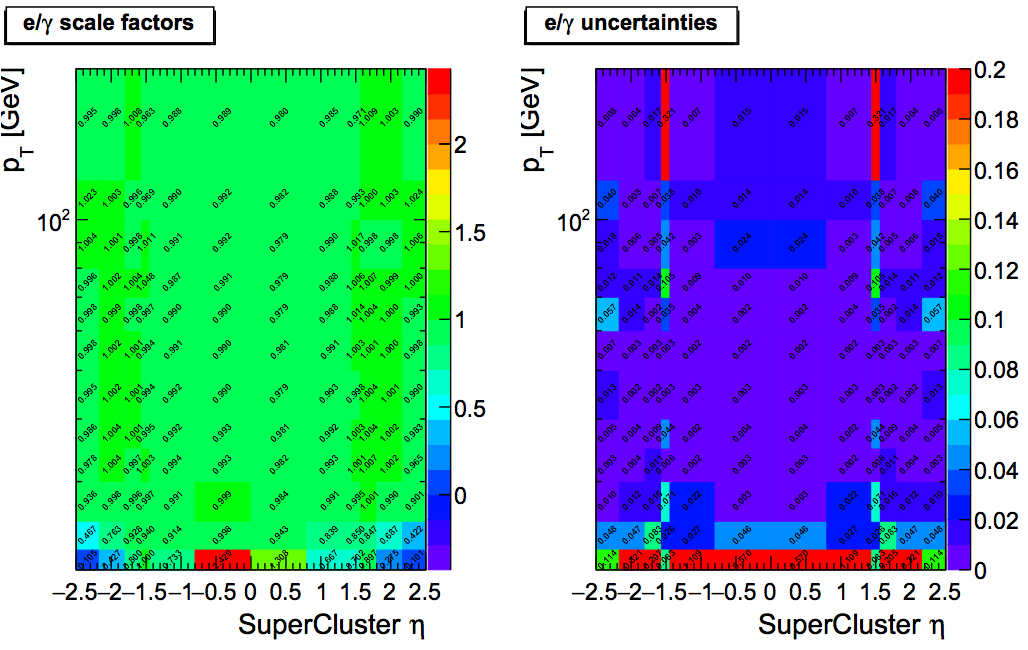
\includegraphics[width=1.0\textwidth]{trigger/electronTriggerEfficiencyelectronTriggerEfficiencyHLT_Leg1_WP90_2016.png} } \\
\subfloat Leg 2
{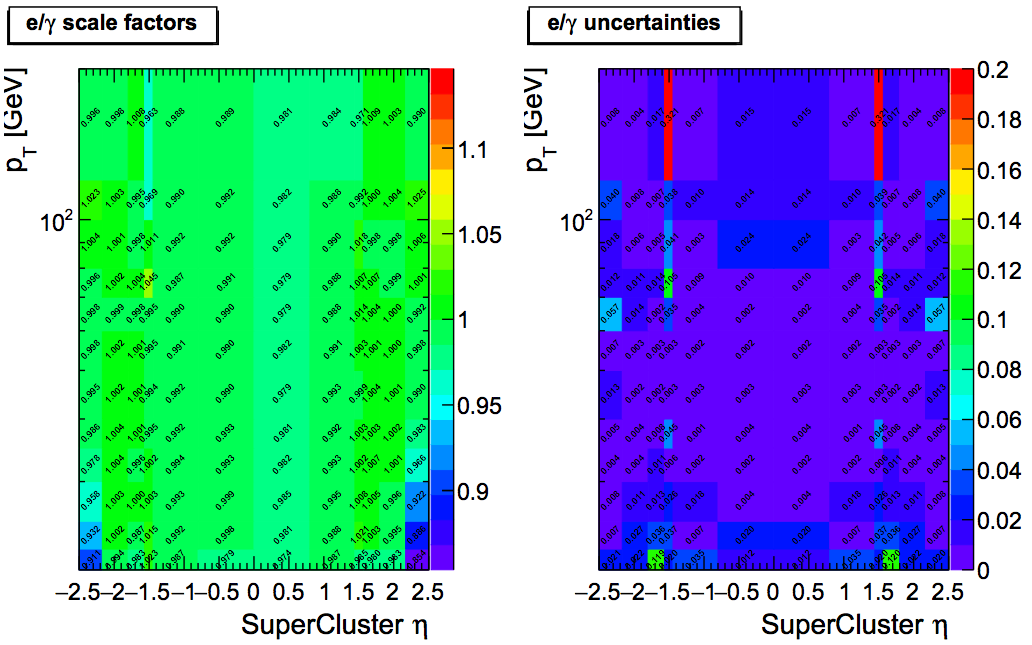
\includegraphics[width=1.0\textwidth]{trigger/electronTriggerEfficiencyelectronTriggerEfficiencyHLT_Leg2_WP90_2016.png} } \\
\caption{Electron scale factors in $p_{T}$ and $\eta$ bins for 2016 data set for the HLT\_Ele23\_Ele12\_CaloIdL\_TrackIdL\_IsoVL\_DZ trigger. ID cut (general purpose MVA WP90) and ISO cuts are applied, then the scale factors are measured. Taken from ~\cite{vhbbAN}}
\label{fig:trigger_eff_diele}
\end{figure}


\begin{figure}
\centering
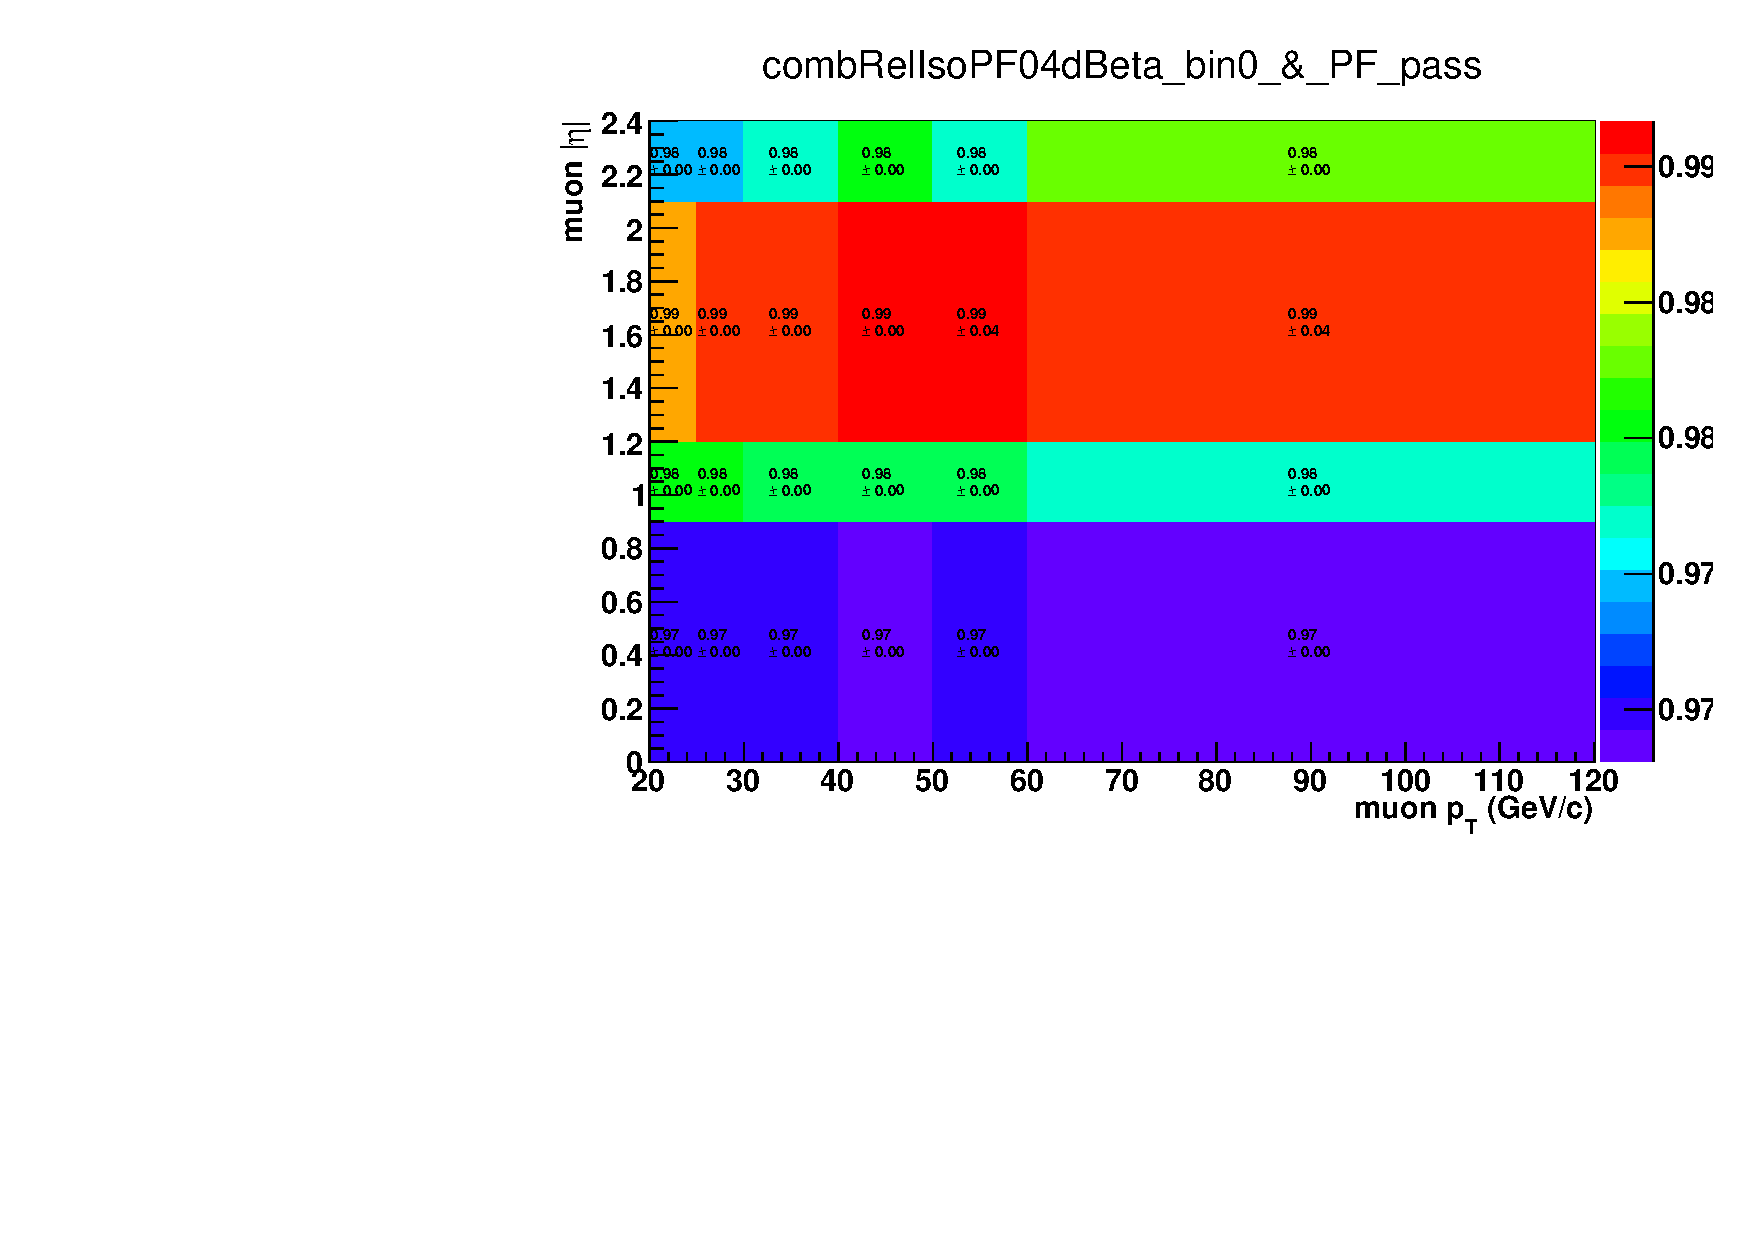
\includegraphics[width=0.475\textwidth]{trigger/Run_BCDEFG_PlotSF_hlt_Mu17_Mu8_OR_TkMu8_leg8_NUM_hlt_Mu17_Mu8_OR_TkMu8_leg8_DEN_LooseIDnISO_PAR_pt_eta_pt_abseta_ratio.pdf}
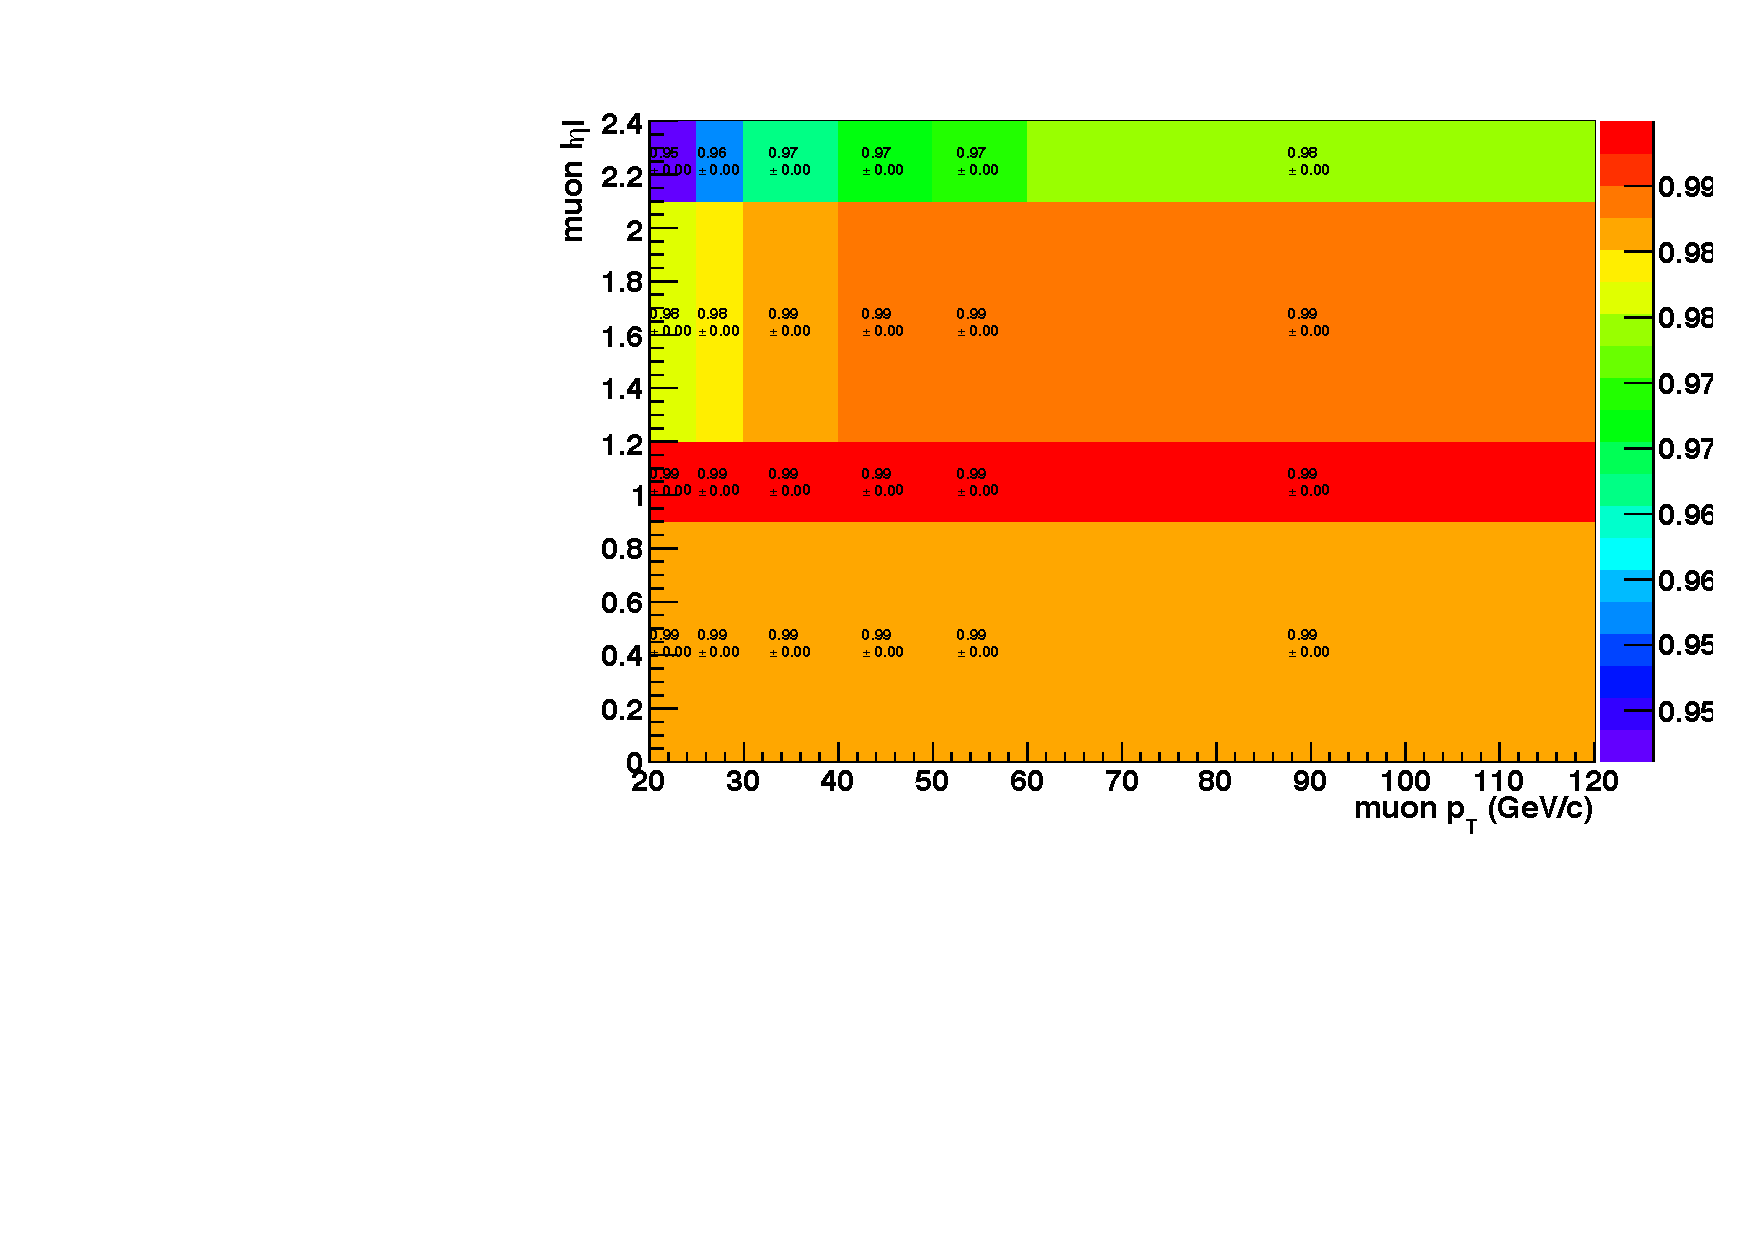
\includegraphics[width=0.475\textwidth]{trigger/Run_BCDEFG_PlotSF_hlt_Mu17Mu8_leg17_NUM_hlt_Mu17Mu8_leg17_DEN_LooseIDnISO_PAR_pt_eta_pt_abseta_ratio.pdf}\\
\caption{Muon scale factors in $p_{T}$ and $\eta$ bins for 2016 data runs B, C, D, E, F, G for the  HLT\_Mu17\_TrkIsoVVL\_Mu8\_TrkIsoVVL\_v* OR HLT\_Mu17\_TrkIsoVVL\_TkMu8\_TrkIs\
oVVL\_v* triggers. Left: Scale factors for 8 GeV leg. Right: Scale factors for 17 GeV leg, provided that the subleading leg passed 8 GeV cut.}
\label{fig:trigger_SF_dimu_BCDEFG}
\end{figure}

\begin{figure}
\centering
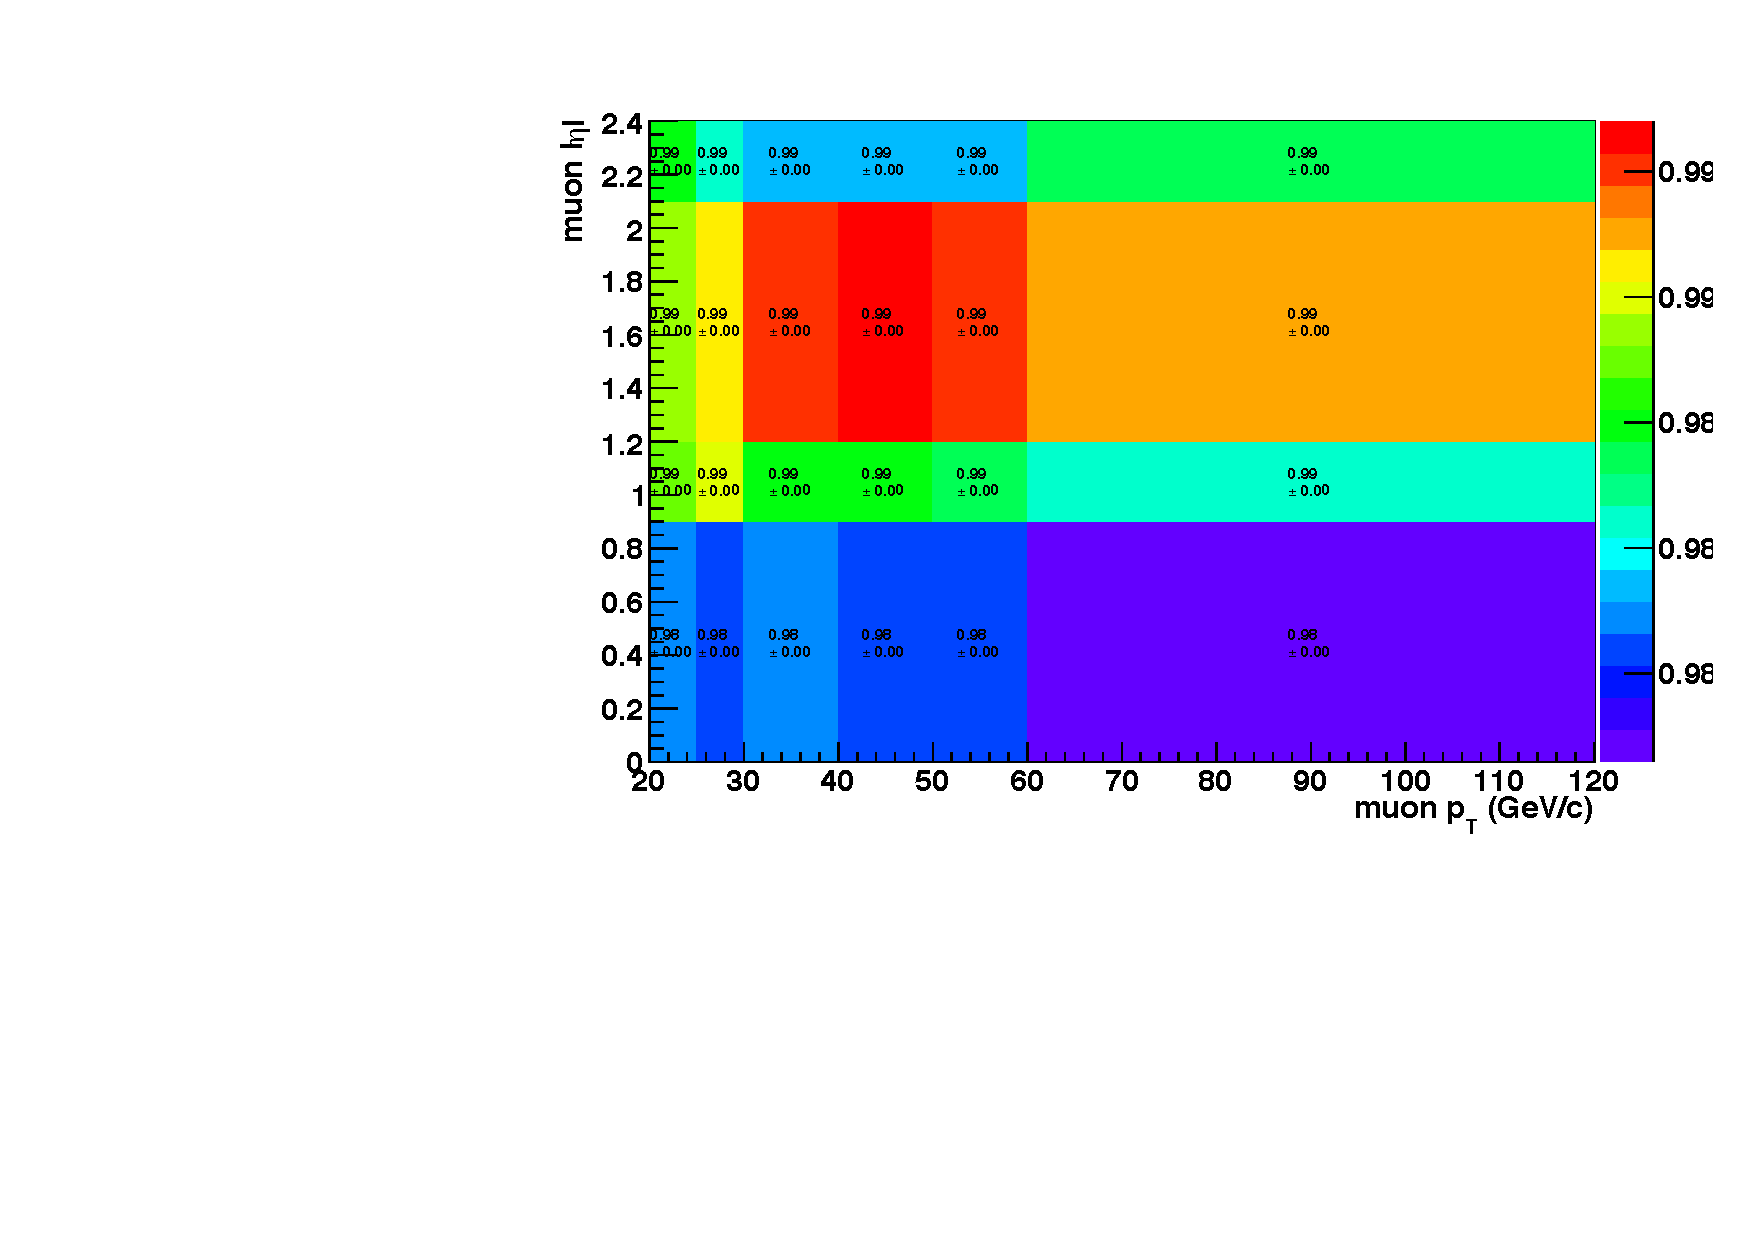
\includegraphics[width=0.475\textwidth]{trigger/Run_H_PlotSF_hlt_Mu17_Mu8_OR_TkMu8_leg8_NUM_hlt_Mu17_Mu8_OR_TkMu8_leg8_DEN_LooseIDnISO_PAR_pt_eta_pt_abseta_ratio.pdf}
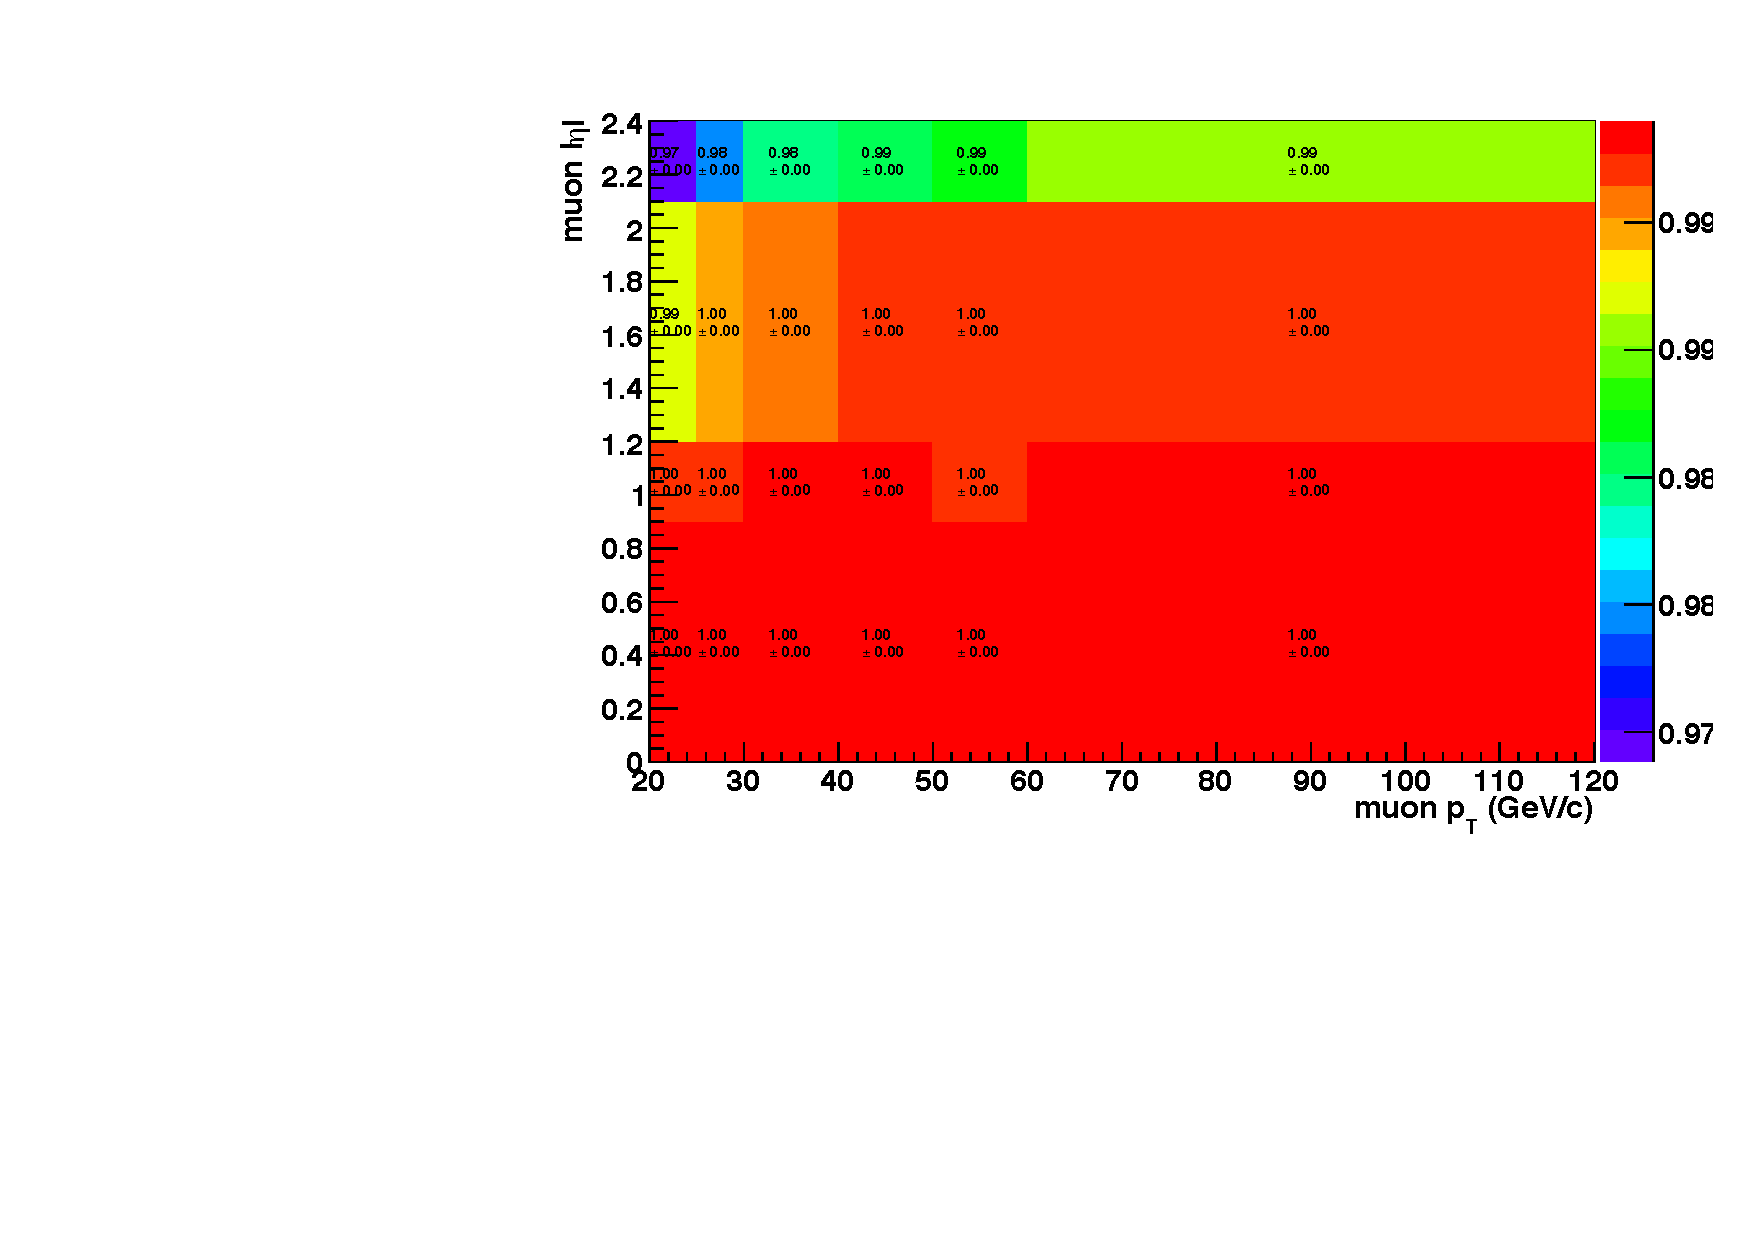
\includegraphics[width=0.475\textwidth]{trigger/Run_H_PlotSF_hlt_Mu17Mu8_leg17_NUM_hlt_Mu17Mu8_leg17_DEN_LooseIDnISO_PAR_pt_eta_pt_abseta_ratio.pdf}\\
\caption{Muon scale factors in $p_{T}$ and $\eta$ bins for 2016 data run H for the  HLT\_Mu17\_TrkIsoVVL\_Mu8\_TrkIsoVVL\_v* OR HLT\_Mu17\_TrkIsoVVL\_TkMu8\_TrkIs\
oVVL\_v* triggers. Left: Scale factors for 8 GeV leg. Right: Scale factors for 17 GeV leg, provided that the subleading leg passed 8 GeV cut.}

\label{fig:trigger_SF_dimu_H}
\end{figure}

\begin{figure}
\centering
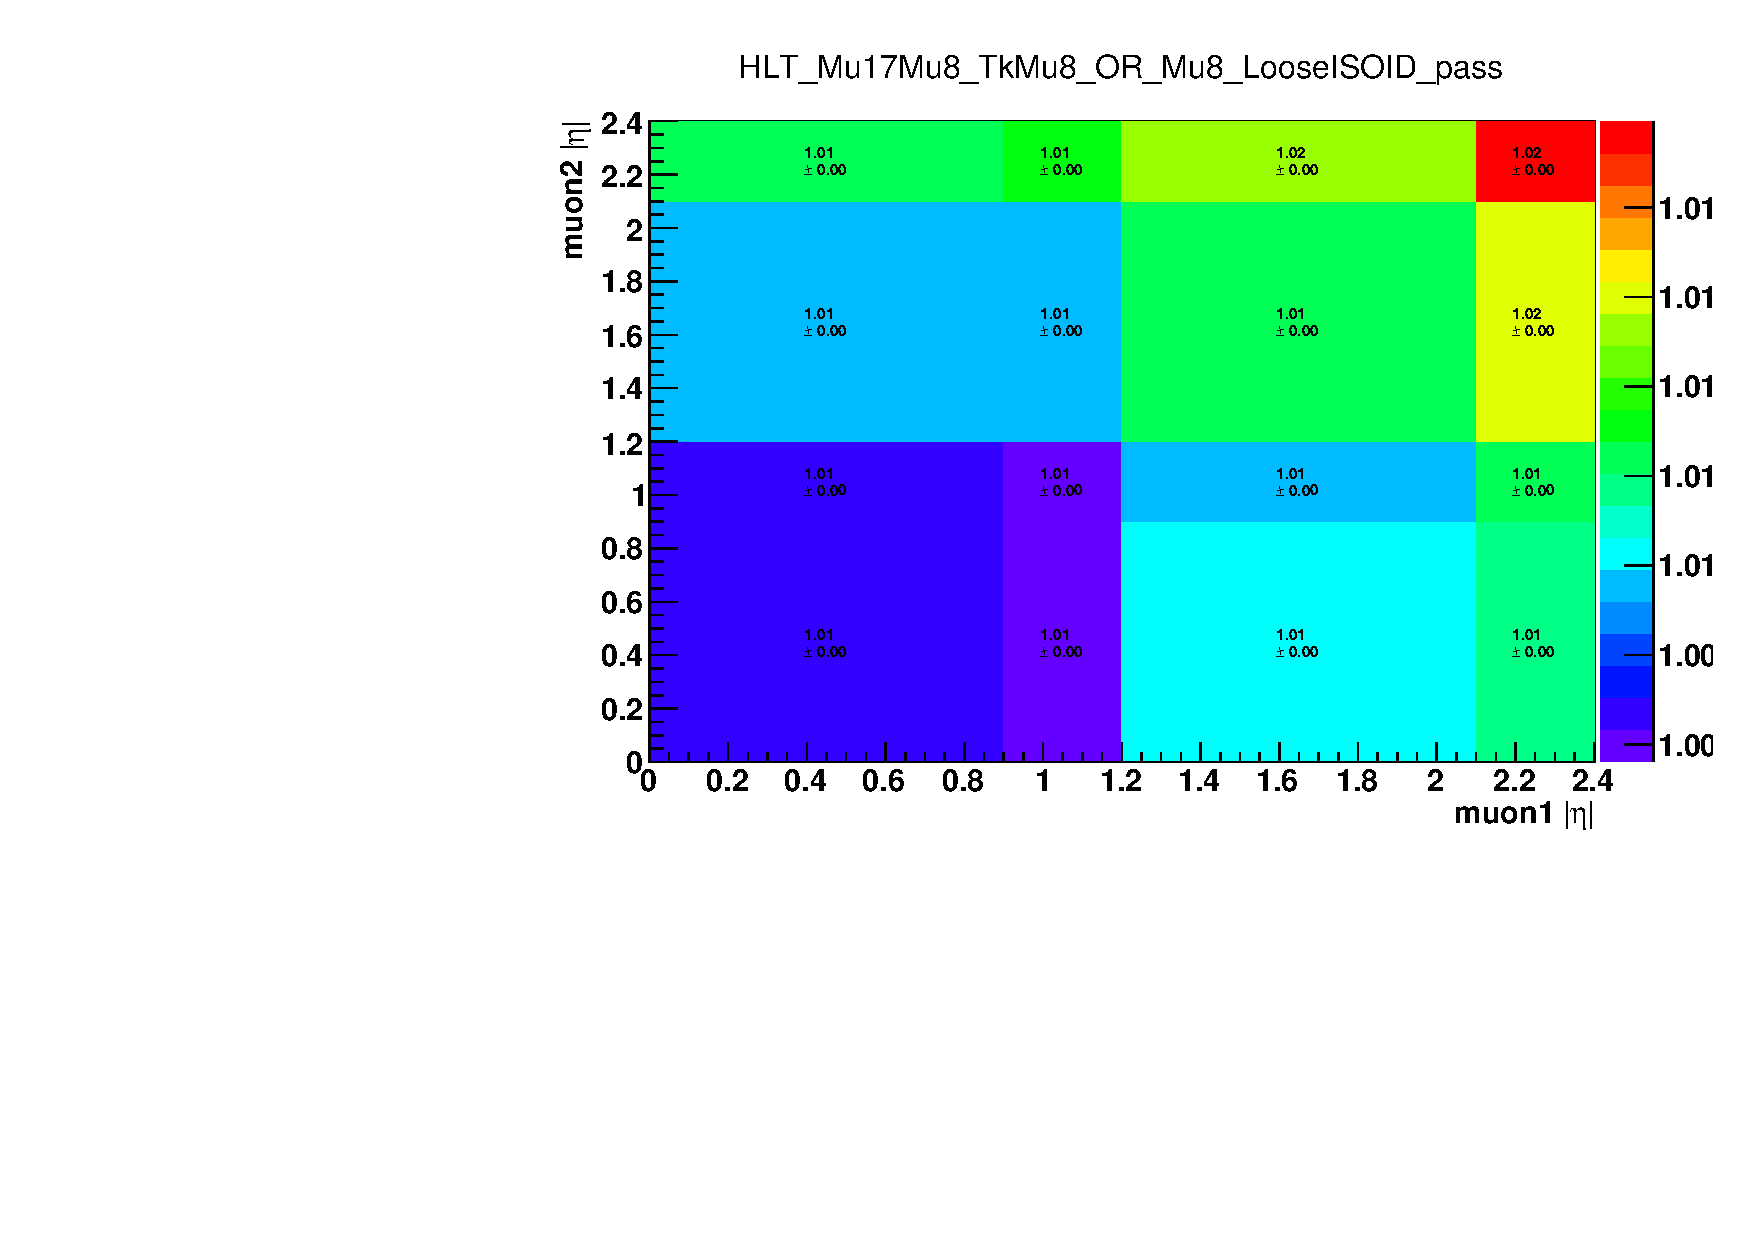
\includegraphics[width=0.85\textwidth]{trigger/PlotSF_dZ_NUM_dZ_DEN_hlt_Mu17_Mu8_OR_TkMu8_loose_PAR_eta1_eta2_abseta_tag_abseta_ratio.pdf}
\caption{Scale factors in $\eta$ bins of the leading and subleading muons for 2016 data set for dZ requirement, measured after muons have passed the HLT\_Mu17\_TrkIsoVVL\_Mu8\_TrkIsoVVL\_v* OR HLT\_Mu17\_TrkIsoVVL\_TkMu8\_TrkIsoVVL\_v* triggers. }
\label{fig:trigger_SF_dimu_dZ_H}
\end{figure}



\begin{figure}
\centering
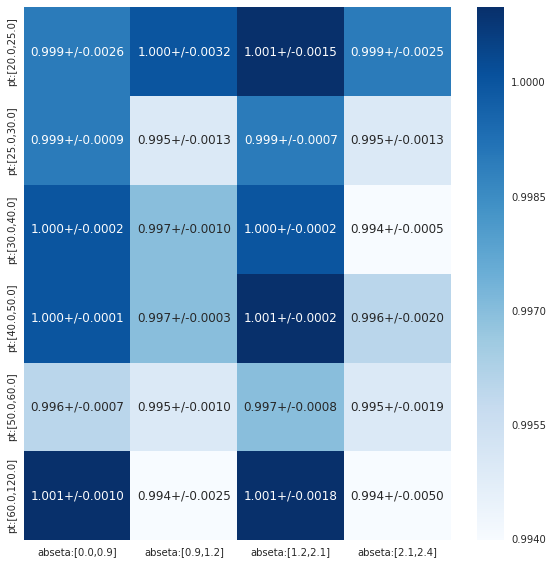
\includegraphics[width=0.5\textwidth]{muon_ID_BCDEFv2.png}
\bigbreak
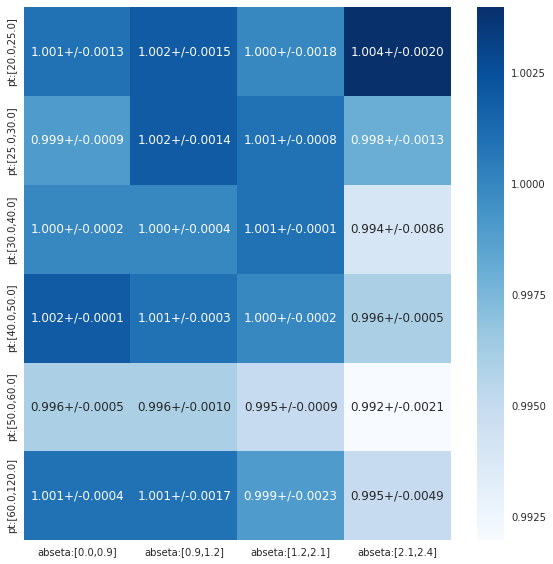
\includegraphics[width=0.5\textwidth]{muon_ID_GHv2.png}
\caption{ Muon ID scale factors in $p_{T}$ and $\eta$ bins. Left: runs B to F. Right: runs G and H.}
\label{fig:muonID_SF}
\end{figure}

\newline
\newline

\begin{figure}
\centering
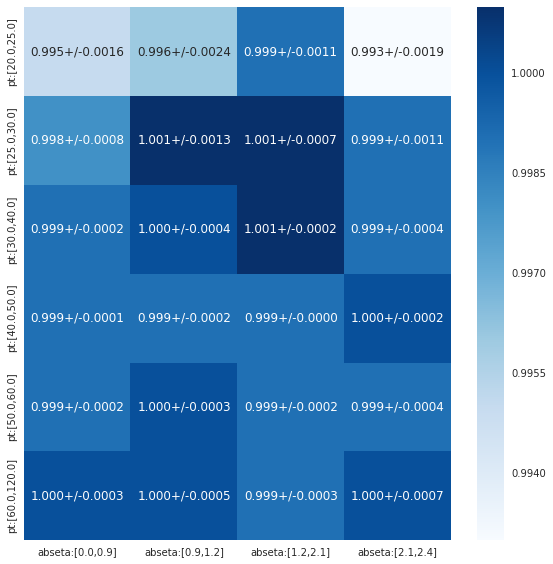
\includegraphics[width=0.5\textwidth]{muon_ISO_BCDEFv2.png}
\bigbreak
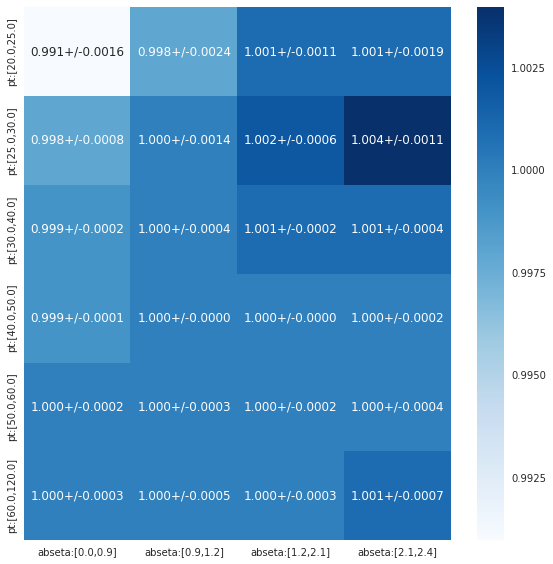
\includegraphics[width=0.5\textwidth]{muon_ISO_GHv2.png}
\caption{ Muon ISO scale factors in $p_{T}$ and $\eta$ bins. Left: runs B to F. Right: runs G and H.}
\label{fig:muonISO_SF}
\end{figure}

\newline
\newline

\begin{figure}
\centering
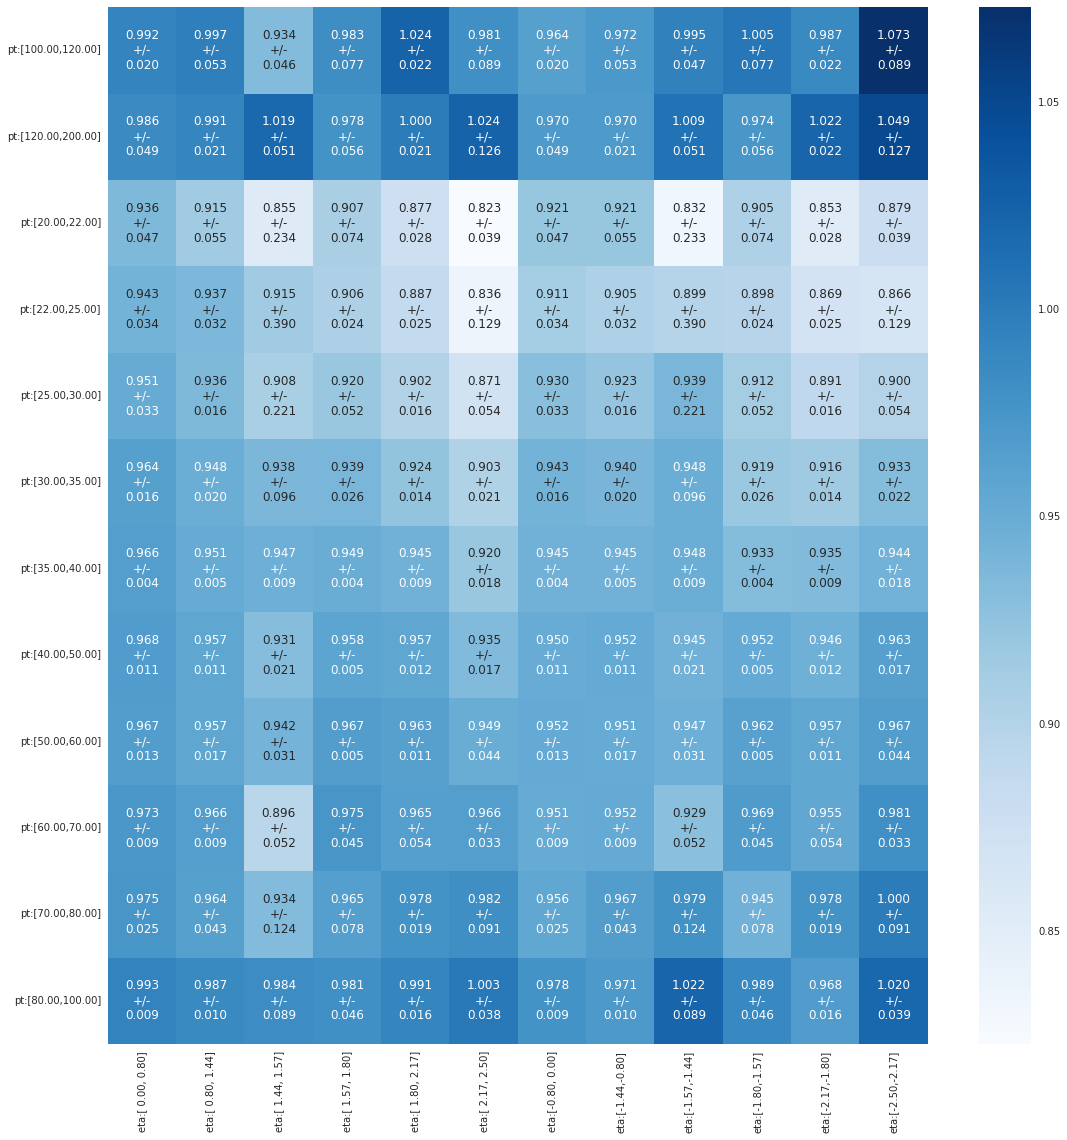
\includegraphics[width=0.9\textwidth]{EIDISO_ZH_out.png}
\caption{ Electron ID+ISO scale factors in $p_{T}$ and $\eta$ bins.}
\label{fig:muonID_SF}
\end{figure}

